\section{Event Loop e Callback Queue}
Fino ad ora abbiamo visto come JavaScript esegua le operazioni in modo sincrono, ovvero una dopo l'altra. 
Questo comportamento è dovuto al fatto che il JavaScript è un linguaggio \textbf{sincrono e single-threaded}, ovvero
esegue un solo task alla volta. Quando un Execution Context viene inserito nello Stack, viene eseguito immediatamente,
e quando termina, viene rimosso dallo Stack.
Tuttavia, ci sono delle operazione che hanno la necessità di essere eseguite in modo asincrono, come ad esempio le operazioni di fetch, setTimeout, setInterval, che possono richiedere molto tempo per essere completate, ma anche l'esecuzione di eventi come il click di un bottone, che non devono essere eseguite immediatamente.
In questi casi, JavaScript non può permettersi di bloccare l'interfaccia utente, quindi deve trovare un modo per gestire queste operazioni in modo asincrono.

\vspace{5mm}
\begin{figure}[H]
    \centering
    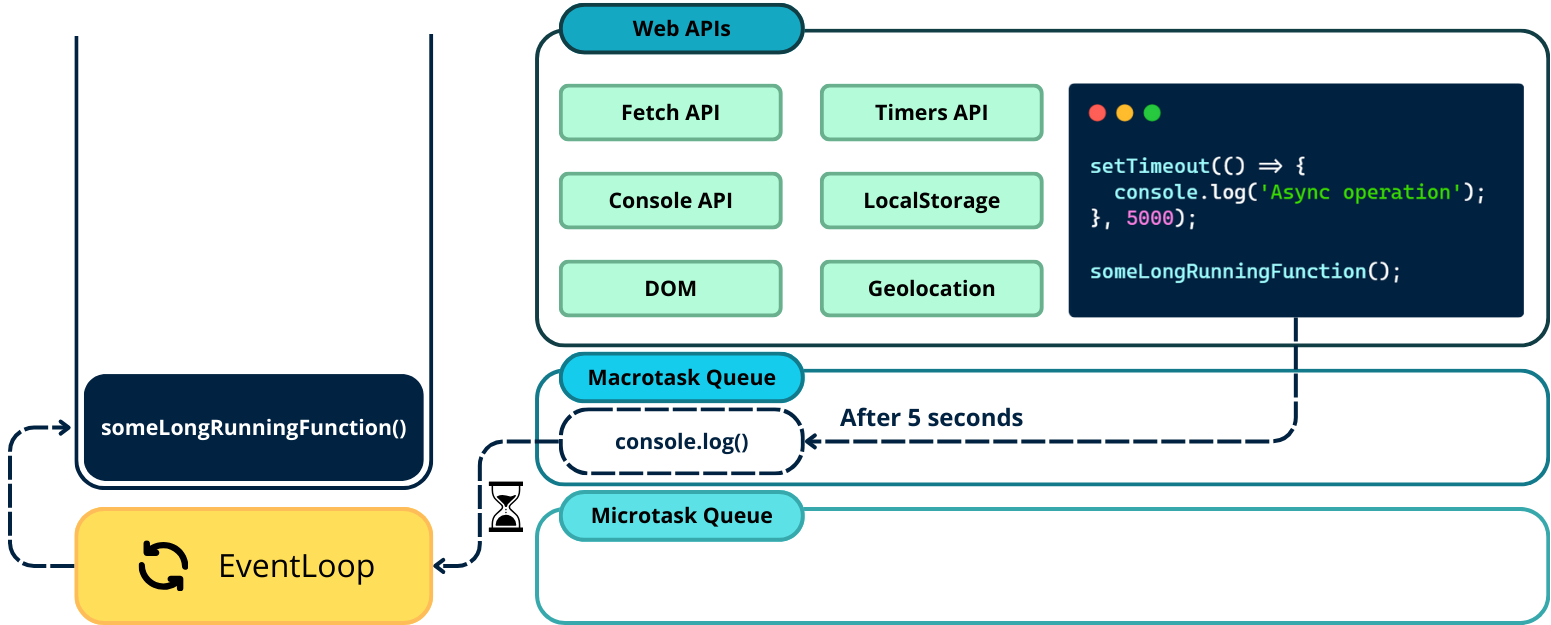
\includegraphics[width=\textwidth]{javascript/eventloop.png}
    \caption{Event Loop e Callback Queue}
    \label{fig:eventloop}
\end{figure}

\subsection{Event Loop}
Per gestire le operazioni asincrone, JavaScript utilizza un meccanismo chiamato \textbf{Event Loop}. L'Event Loop è un componente che implementa il pattern \emph{Observer}, che si occupa di monitorare lo Stack e la Callback Queue, e di spostare le funzioni dalla Callback Queue allo Stack quando lo Stack è vuoto. In questo modo, JavaScript può eseguire le operazioni asincrone senza bloccare l'interfaccia utente.
Questo spostamento però avviene solo quando lo Stack è vuoto, quindi le funzioni asincrone vengono eseguite solo dopo che tutte le funzioni sincrone sono state completate. Questo garantisce che le funzioni asincrone non interferiscano con le funzioni sincrone, e che l'interfaccia utente rimanga reattiva.

\subsection{Callback Queue}
La Callback Queue è una coda in cui vengono inserite le funzioni che devono essere eseguite in modo asincrono. Quando una funzione asincrona viene completata, viene inserita nella Callback Queue, in attesa di essere eseguita. Quando lo Stack è vuoto, l'Event Loop prende la funzione in testa alla Callback Queue e la sposta nello Stack, dove viene eseguita.
La callback Queue è in realtà formata da due code: la \textbf{MacroTask Queue} e la \textbf{MicroTask Queue}. La MacroTask Queue contiene le funzioni asincrone di livello più alto, come ad esempio le operazioni di fetch, setTimeout, setInterval, mentre la MicroTask Queue contiene le funzioni asincrone di livello più basso, ovvero le Promises. Le funzioni della MicroTask Queue vengono eseguite prima di quelle della MacroTask Queue, in modo da garantire che le Promises vengano risolte prima delle altre operazioni asincrone. 

\subsection{Esempio}
Prendiamo per esempio il codice in figura \ref{fig:eventloop} per capire meglio come funziona questo meccanismo.

Quando il codice viene eseguito, i passaggi sono i seguenti:
\begin{itemize}
  \item Il JavaScript Engine parsa il codice e riconosce la funzione setTimeout. Questa funzione serve ad eseguire una funzione in modo asincrono dopo un certo intervallo di tempo. In questo caso, la funzione setTimeout esegue la funzione console.log() dopo 5 secondi.
  \item A questo punto, il JavaScript runtime crea un nuovo thread, che si occupa di gestire la funzione setTimeout. Questo thread si occupa di contare i 5 secondi e di inserire la funzione console.log() nella MacroTask Queue quando il tempo è scaduto.
  \item Nel frattempo, il JavaScript Engine esegue la funzione someLongRunningFunction(). Questa funzione è una funzione sincrona fittizia che richiede molto tempo per essere completata. 
\end{itemize}

Quando la funzione \texttt{someLongRunningFunction()} viene completata, il JavaScript Engine rimuove la funzione dallo Stack. A questo punto, l'Event Loop, che osserva costantemente lo Stack, nota che lo Stack è vuoto, prende la funzione \emph{ console.log()} dalla MacroTask Queue e la sposta nello Stack, dove viene eseguita. In questo modo, la funzione \emph{console.log()} viene eseguita dopo che la funzione \texttt{someLongRunningFunction()} è stata completata.

È importante notare però, che 5 secondi non è il tempo esatto dopo la quale la funzione verrà eseguita. Infatti questo è il tempo dopo il quale la funzione verrà inserita nella MacroTask Queue. Se la funzione \texttt{someLongRunningFunction()} richiede più di 5 secondi per essere completata, la funzione \emph{console.log()} verrà effettivamente eseguita dopo un tempo maggiore di quello previsto. Questo è un aspetto importante da tenere in considerazione quando si scrive codice JavaScript asincrono.